\documentclass[12pt]{book}

\usepackage{graphicx} % Required for inserting images
\usepackage{geometry}  % Per modificare i margini
\usepackage{setspace} %per l'interlinea

\usepackage[utf8]{inputenc}  % Per gli accenti
\usepackage[italian]{babel}  % Per la lingua
\usepackage{lipsum}          % Testo fittizio  
% \usepackage{indentfirst}     % Fa partire i paragrafi col rientro
\usepackage{hyperref}        % Per link cliccabili nell'indice
\usepackage[normalem]{ulem} % per sottolineare
\usepackage{soul}     % Per evidenziare testo
\usepackage{xcolor}   % Per i colori
\usepackage{wrapfig}    % testo attorno alle immagini
\usepackage{caption}    % per caption fuori dalle float
% \captionsetup{hypcap=false} % Disabilita hypcap per evitare warning con \captionof
\usepackage{floatrow}   % per floatrow

\setcounter{secnumdepth}{4} % Imposta il livello massimo di sezioni che verranno numerate.
                            % 0 = \part
                            % 1 = \section
                            % 2 = \subsection
                            % 3 = \subsubsection
                            % 4 = \paragraph
                            % 5 = \subparagraph (se disponibile)
                            
\setcounter{tocdepth}{4}    % Imposta il livello massimo di sezioni che verranno mostrate nell'indice (table of contents).
                            % Stessi livelli di sopra: 4 = mostra fino ai \paragraph nell'indice.





% Margini personalizzati
\geometry{
  a4paper,
  left=2cm,
  right=2cm,
  top=2cm,
  bottom=2cm
}


\begin{document}

\begin{titlepage}
    \centering
    \vspace*{4cm}
    {\LARGE\textbf{Relazione per l'esame di }\par}
    {\LARGE\textbf{Informatica Giuridica}\par}
    \vspace{4cm}
    {\Large\textbf{Argomento: Hate Speech}\par}
    \vspace{1cm}
    \vfill
    {\large Studente: Antonio Runcio\par}
    \vspace{0.5cm}
    {\large Agosto 2025\par}
    \thispagestyle{empty} % niente numero di pagina qui
\end{titlepage}



\section*{Formattazione del testo}
\textit{Testo corsivo}

\textbf{Testo in grassetto}

\underline{Testo sottolineato}

\sout{Testo barrato} % barrato

\uline{Testo sottolineato con ulem} % sottolineato con ulem

\uwave{Testo sottolineato ondulato} % sottolineato ondul

\newpage

\section*{Evidenziatore in LaTeX}

\subsection*{1. Evidenziatore giallo (default)}
Questo è un testo \hl{evidenziato in giallo}.

\subsection*{2. Cambiare colore dell'evidenziatore}

\textbf{Azzurro:}\\
{\sethlcolor{cyan!30}\hl{Testo evidenziato in azzurro}}

\vspace{5pt}
\textbf{Rosa:}\\
{\sethlcolor{pink}\hl{Testo evidenziato in rosa}}

\vspace{5pt}
\textbf{Verde chiaro:}\\
{\sethlcolor{green!30}\hl{Testo evidenziato in verde chiaro}}

\vspace{5pt}
\textbf{Arancione:}\\
{\sethlcolor{orange!40}\hl{Testo evidenziato in arancione}}

\subsection*{3. Evidenziare in modalità matematica}

\textbf{Formula evidenziata:}\\
\colorbox{yellow}{$E = mc^2$}

\vspace{5pt}
\colorbox{cyan!30}{$\int_0^1 x^2\,dx$}

\subsection*{4. Legenda colori (modificabili)}

\begin{itemize}
  \item \texttt{yellow} = giallo
  \item \texttt{cyan!30} = azzurro
  \item \texttt{pink} = rosa
  \item \texttt{green!30} = verde chiaro
  \item \texttt{orange!40} = arancione
  \item ... puoi usare anche \texttt{red}, \texttt{blue!20}, \texttt{purple!40}, ecc.

  
\end{itemize}

\newpage

\section*{1. Metodo con wrapfig (testo che scorre attorno)}
\begin{wrapfigure}{r}{0.7\textwidth}
  \centering
  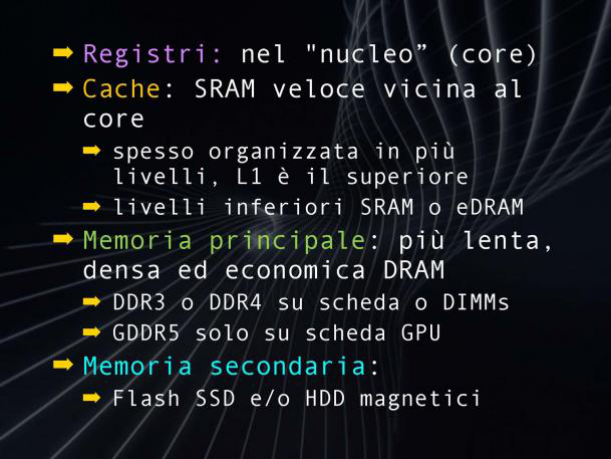
\includegraphics[width=0.95\textwidth]{images/Lez06_p02_fig_01.png}
  \caption{Esempio wrapfig}
\end{wrapfigure}
\lipsum[1-2] % testo lungo fittizio

\newpage

\section*{2. Metodo con minipage (blocco affiancato, NO scorrimento)}
\noindent
\begin{minipage}{0.5\textwidth}
\lipsum[3-4] % testo lungo a sinistra
\end{minipage}%
\hfill
\begin{minipage}{0.5\textwidth}
\centering

\includegraphics[width=\linewidth]{images/Lez01_p01_fig_01.png}
\captionof{figure}{Esempio minipage}
\end{minipage}

\newpage

\section*{3. Metodo con floatrow (più elegante, immagine e caption a lato)}

\lipsum[9-10] % testo lungo fittizio
\begin{figure}[h]
\floatbox[{\capbeside\thisfloatsetup{capbesideposition={center,center}}}]{figure}[\FBwidth]
{\caption{Esempio floatrow}}
{
\includegraphics[width=0.5\textwidth]{images/Lez01_p01_fig_01.png}}
\end{figure}

\lipsum[5-6] % testo lungo fittizio




\end{document}